% !Mode:: "TeX:UTF-8"
\documentclass[newtxmath=true,newgeometry=two,capcenterlast=true,subcapcenterlast=true,openright=false,library=false,absupper=true,fontset=windowsnew,type=doctor]{hithesis}
% 此处选项中不要有空格
%%%%%%%%%%%%%%%%%%%%%%%%%%%%%%%%%%%%%%%%%%%%%%%%%%%%%%%%%%%%%%%%%%%%%%%%%%%%%%%%
% 必填选项
% type=doctor|master|bachelor
%%%%%%%%%%%%%%%%%%%%%%%%%%%%%%%%%%%%%%%%%%%%%%%%%%%%%%%%%%%%%%%%%%%%%%%%%%%%%%%%
% 选填选项(选填选项的缺省值已经尽可能满足了大多数需求,除非明确知道自己有什么
% 需求)
% glue=true|false
% 	含义:由于我工规范中要求字体行距在一个闭区间内,这个选项为true表示tex自
% 	动选择,为false表示区间内一个最接近版心要求行数的要求的默认值,缺省值为
% 	false。
% tocfour=true|false
% 	含义:是否添加第四级目录,只对本科文科个别要求四级目录有效,缺省值为
% 	false
% fontset=siyuan|windowsnew|windowsold
% 	含义:注意这个选项视为了解决特殊问题而设置,比如用有些发行版本的linux排
% 	版时可能(大多数发行版不会)会遇到的字体无法载入的问题,或者字体载入之
% 	后出现无法复制的问题以及想要解决排版如 biang biang 面的 biang 这类中易
% 	宋体无法识别的汉字的问题。没有特殊的需要不推荐使用这个选项。
%
% 	如果是安装了 windows 字体的 linux 系统,可以填写windowsnew(win vista
% 	以后 的字体)或 windowsold(vista 以前)或者想用思源宋体并且是已经安装
% 	了思源宋体的任何系统,填写siyuan选项。缺省值为空,自动识别系统并匹配字体
% 	。模板版中给出的思源字体定义文件定义的思源字体的版本是Adobe版,其他字体
% 	是windowsnew字体。
% tocblank=true|false
% 	含义:目录中第一章之前,是否加一行空白。缺省值为true。
% chapterhang=true|false
% 	含义:目录的章标题是否悬挂居中,规范中要求章标题少于15字,所以这个选项
% 	有无没什么用,除了特殊需求。缺省值为true。
% fulltime=true|false
% 	含义:是否全日制,缺省值为true。非全日制如同等学力等,要在cover中设置类
% 	型,封面中不同格式
% subtitle=true|false
% 	含义:论文题目是否含有副标题,缺省值为false,如果有要在cover中设置副标
% 	题内容,封面中显示。
% newgeometry=one|two
% 	含义:规范中的自相矛盾之处,版芯是否包含页眉页脚,旧方法是按照包含页眉
% 	页脚来设置。该选项是多选选项,如果没有这个选项,缺省值是旧模板的版芯设
% 	置方法,如果设置该选项one或two,分别对应两种页眉页码对应版芯线的相对位
% 	置。第一种是严格按照规范要求,难看。第二种微调了页眉页码位置,好一点。
% debug=true|false
% 	含义:是否显示版芯框和行号,用来调试。默认否。
% openright=true|false
% 	含义:博士论文是否要求章节首页必须在奇数页,此选项不在规范要求中,按个
% 	人喜好自行决定。 默认否。注意,窝工的默认情况是打印版博士论文要求右翻页
% 	,电子版要求非右翻页且无空白页。如果想DIY(或身不由己DIY)在什么地方右
% 	翻页,将这个选项设置为false,然后在目标位置添加`\cleardoublepage`命令即
% 	可。
% library=true|false
%   含义:是否为提交到图书馆的电子版。默认否。注意:如果设置成true,那么
%   openright选项将被强制转换为false。
% capcenterlast=true|false
% 	含义:图题、表题最后一行是否居中对齐(我工规范要求居中,但不要求居中对
% 	齐),此选项不在规范要求中,按个人喜好自行决定。默认否。
% subcapcenterlast=true|false
% 	含义:子图图题最后一行是否居中对齐(我工规范要求居中,但不要求居中对齐
% 	),此选项不在规范要求中,按个人喜好自行决定。默认否。
% absupper=true|false
%   含义:中文目录中的英文摘要在中文目录中的大小写样式歧义,在规范中要求首
%   字母大写,在work样例中是全大写。该选项控制是否全大写。默认否。
% bsmainpagenumberline=true|false
%   含义:由于本科生论文官方模板的页码和页眉格式混乱,提供这个选项自定义设
%   置是否在正文中显示页码横线,默认否。
% bsfrontpagenumberline=true|false
%   含义:由于本科生论文官方模板的页码和页眉格式混乱,提供这个选项自定义设
%   置是否在前文中显示页码横线,默认否。
% bsheadrule=true|false
%   含义:由于本科生论文官方模板的页码和页眉格式混乱,提供这个选项自定义设
%   置是否显示页眉横线,默认显示。
% splitbibitem=true|false
%   含义:参考文献每一个条目内能不能断页,应广大刀客要求添加。默认否。
% newtxmath=true|false
%   含义:数学字体是否使用新罗马。默认是。
%%%%%%%%%%%%%%%%%%%%%%%%%%%%%%%%%%%%%%%%%%%%%%%%%%%%%%%%%%%%%%%%%%%%%%%%%%%%%%%%

\usepackage{hithesis}
\graphicspath{{figures/}}

\begin{document}

\frontmatter
\cqusetup{
%	************	注意	************
%	* 1. \cqusetup{}中不能出现全空的行,如果需要全空行请在行首注释
%	* 2. 不需要的配置信息可以放心地坐视不理、留空、删除或注释(都不会有影响)
%	*
%	********************************
% ===================
%	论文的中英文题目
% ===================
  ctitle = {\ce{C60}表面的纳米形貌的可控性转变\\兼论\LaTeX{}在论文排版中的运用},
  etitle = {To Use \LaTeX{} in the Typeseting of\\Graduating Work for CQU},
% ===================
% 作者部分的信息
% \secretize{}为盲审标记点,在打开盲审开关时内容会自动被替换为***输出,盲审开关默认关闭
% ===================
  cauthor = \secretize{李振楠},	% 你的姓名,以下每项都以英文逗号结束
  eauthor = \secretize{Zhennan~Li},	% 姓名拼音,~代表不会断行的空格
  studentid = \secretize{20128888},	% 仅本科生,学号
  csupervisor = \secretize{孙麟~~教授},	% 导师的姓名
  esupervisor = \secretize{{Prof.~Lin Sun}},	% 导师的姓名拼音
  cassistsupervisor = \secretize{}, % 本科生可选,助理指导教师姓名,不用时请留空为{}
  cextrasupervisor = \secretize{}, % 本科生可选,校外指导教师姓名,不用时请留空为{}
  eassistsupervisor = \secretize{}, % 本科生可选,助理指导教师或/和校外指导教师姓名拼音,不用时请留空为{}
  cpsupervisor = \secretize{丁小明~~工程师}, % 仅专硕,兼职导师姓名
  epsupervisor = \secretize{Eng.~Xiaoming~Ding},	% 仅专硕,兼职导师姓名拼音
  cclass = 工学,	% 博士生和学硕填学科门类,学硕填学科类型
  edgree = {Degree of Master of Enginnering},	% 专硕填Professional Degree,其他按实情填写
% 提示:如果内容太长,可以用\zihao{}命令控制字号,作用范围:{}内
  cmajor = {\zihao{-4}材料科学与工程(材料科学专业方向)},	% 专硕不需填,填写专业名称
  emajor = Material Science and Engineering, % % 专硕不需填,填写专业英文名称
% ===================
% 底部的学院名称和日期
% ===================
  cdepartment = 材料科学与工程学院,	%学院名称
  edepartment = College of Material Science and Engineering,	%学院英文名称
% ===================
% 封面的日期可以自动生成(注释掉时),也可以解除注释手动指定,例如:二〇一六年五月
% ===================
%	mycdate = {中文日期},
%	myedate = {Date in English},
}% End of \cqusetup
% ===================
%
% 论文的摘要
%
% ===================
\begin{cabstract}	% 中文摘要
	本文档是\cquthesis{}的示例文档。
		
	\cquthesis{}是重庆大学毕业论文的\LaTeX{}模板,支持学士、硕士、博士论文的排版。合理使用本模板可以大大减轻重庆大学毕业生在毕业论文撰写过程中的排版工作量。
	
	\cquthesis{}根据重庆大学《重庆大学本科设计(论文)撰写规范化要求(2007年修订版)》和《重庆大学博士、硕士论文撰写格式标准(2007年修订版)》编写,力求合规,简洁,易于实现,用户友好。
	
	本模板的特色:
  \begin{itemize}
  	\item 支持重庆大学本科(文学、理工)、硕士(学术、专业)、博士的毕业论文格式;
  	\item 内置封面、目录、索引、授权书等论文部件,可按需自动生成;
  	\item 自动侦测文档页数,生成相应的单面打印/双面打印PDF文件;
  	\item 预置一批优化过的宏包和小功能,包含国际标准单位、化学式支持、三线表等,可按需开启。
  \end{itemize}
\end{cabstract}
% 中文关键词,请使用英文逗号分隔:
\ckeywords{重庆大学,\LaTeX,\LaTeXe,论文,模板}

\begin{eabstract}	% 英文摘要
	LaTeX is a document preparation system for high-quality typesetting. It is most often used for medium-to-large technical or scientific documents but it can be used for almost any form of publishing.
	
  LaTeX contains features for:
\begin{enumerate}
  	\item Typesetting journal articles, technical reports, books, and slide presentations.
  	\item Control over large documents containing sectioning, cross-references, tables and figures.
  	\item Typesetting of complex mathematical formulas.
  	\item Advanced typesetting of mathematics with AMS-LaTeX.
  	\item Automatic generation of bibliographies and indexes.
  	\item Multi-lingual typesetting.
  	\item Inclusion of artwork, and process or spot colour.
  	\item Using PostScript or Metafont fonts.
  \end{enumerate}
  (Quote from \textit{https://latex-project.org/intro.html})  
\end{eabstract}
% 英文关键词,请使用英文逗号分隔,关键词内可以空格:
\ekeywords{bachelor, master, doctor, all support, white space is okay here}

% 封面和摘要配置完成
 % 封面
\makecover
% !TeX root = ../main.tex

\begin{denotation}[3cm]
\item[HPC] 高性能计算 (High Performance Computing)
\item[cluster] 集群
\item[Itanium] 安腾
\item[SMP] 对称多处理
\item[API] 应用程序编程接口
\item[PI] 聚酰亚胺
\item[MPI] 聚酰亚胺模型化合物,N-苯基邻苯酰亚胺
\item[PBI] 聚苯并咪唑
\item[MPBI] 聚苯并咪唑模型化合物,N-苯基苯并咪唑
\item[PY] 聚吡咙
\item[PMDA-BDA]	均苯四酸二酐与联苯四胺合成的聚吡咙薄膜
\item[$\increment G$] 活化自由能 (Activation Free Energy)
\item[$\chi$] 传输系数 (Transmission Coefficient)
\item[$E$] 能量
\item[$m$] 质量
\item[$c$] 光速
\item[$P$] 概率
\item[$T$] 时间
\item[$v$] 速度
\item[劝学] 君子曰:学不可以已。青,取之于蓝,而青于蓝;冰,水为之,而寒于水。木
  直中绳。輮以为轮,其曲中规。虽有槁暴,不复挺者,輮使之然也。故木受绳则直,金就
  砺则利,君子博学而日参省乎己,则知明而行无过矣。吾尝终日而思矣,不如须臾之所学
  也;吾尝跂而望矣,不如登高之博见也。登高而招,臂非加长也,而见者远;顺风而呼,
  声非加疾也,而闻者彰。假舆马者,非利足也,而致千里;假舟楫者,非能水也,而绝江
  河,君子生非异也,善假于物也。积土成山,风雨兴焉;积水成渊,蛟龙生焉;积善成德,
  而神明自得,圣心备焉。故不积跬步,无以至千里;不积小流,无以成江海。骐骥一跃,
  不能十步;驽马十驾,功在不舍。锲而舍之,朽木不折;锲而不舍,金石可镂。蚓无爪牙
  之利,筋骨之强,上食埃土,下饮黄泉,用心一也。蟹六跪而二螯,非蛇鳝之穴无可寄托
  者,用心躁也。—— 荀况
\end{denotation}



% % 也可以使用 nomencl 宏包:

% \printnomenclature[3cm]

% \nomenclature{HPC}{高性能计算 (High Performance Computing)}
% \nomenclature{cluster}{集群}
% \nomenclature{Itanium}{安腾}
% \nomenclature{SMP}{对称多处理}
% \nomenclature{API}{应用程序编程接口}
% \nomenclature{PI}{聚酰亚胺}
% \nomenclature{MPI}{聚酰亚胺模型化合物,N-苯基邻苯酰亚胺}
% \nomenclature{PBI}{聚苯并咪唑}
% \nomenclature{MPBI}{聚苯并咪唑模型化合物,N-苯基苯并咪唑}
% \nomenclature{PY}{聚吡咙}
% \nomenclature{PMDA-BDA}{均苯四酸二酐与联苯四胺合成的聚吡咙薄膜}
% \nomenclature{$\increment G$}{活化自由能 (Activation Free Energy)}
% \nomenclature{$\chi$}{传输系数 (Transmission Coefficient)}
% \nomenclature{$E$}{能量}
% \nomenclature{$m$}{质量}
% \nomenclature{$c$}{光速}
% \nomenclature{$P$}{概率}
% \nomenclature{$T$}{时间}
% \nomenclature{$v$}{速度}
%物理量名称表,符合规范为主,有要求添加
%\cleardoublepage  自定义在什么位置进行右翻页
\tableofcontents    % 中文目录
%\cleardoublepage  自定义在什么位置进行右翻页
\tableofengcontents % 英文目录,硕本不要求

\mainmatter
%\linenumbers %debug 选项
%\layout %debug 选项
%\floatdiagram %debug 选项
%\begin{figure} %debug 选项
%\currentfloat %debug 选项
%\tryintextsep{\intextsep} %debug 选项
%\trytopfigrule{0.5pt} %debug 选项
%\trybotfigrule{1pt} %debug 选项
%\setlayoutscale{0.9} %debug 选项
%\floatdesign %debug 选项
%\caption{Float layout with rules}\label{fig:fludf} %debug 选项
%\end{figure} %debug 选项
\documentclass[12pt]{report}
\usepackage[utf8]{inputenc}
\usepackage[brazilian,brazil]{babel}
\usepackage{fancyhdr,setspace,float,graphicx,lscape,array,longtable,colortbl,amsmath,amssymb,booktabs,multirow,hyperref,pdfpages,tocloft,titlesec,lipsum,natbib}
\usepackage[sectionbib]{chapterbib}
\begin{document}
%***
\clearpage
\linenumbers % numeração de linhas
\modulolinenumbers[3] % numeração de linhas
%***
% Texto
%***
\chapter{Nam dui ligula}
%***
\lipsum[2-2] Nam dui ligula, fringilla a, euismod sodales, sollicitudin vel, wisi. Morbi
auctor lorem non justo \citep{lamport1986latex}.
\section{Euismod sodales}
\lipsum[2-3]
%*** APAGAR O EXEMPLO ACIMA







%*** REFERÊNCIAS
\bibliography{referencias.bib}
\bibliographystyle{apalike}
\end{document}


\backmatter
%硕博书序
\chapter{The conclusion}

   % 结论
\bibliographystyle{hithesis} %如果没有参考文献时候
\bibliography{reference}
\begin{appendix}%附录
% -*-coding: utf-8 -*-
%%%%%%%%%%%%%%%%%%%%%%%%%%%%%%%%%%%%%%%%%%%%%%%%%%%%%%%%%
\chapter{带章节的附录}[Full Appendix]%
完整的附录内容,包含章节,公式,图表等

%%%%%%%%%%%%%%%%%%%%%%%%%%%%%%%%%%%%%%%%%%%%%%%%%%%%%%%%%
\section{附录节的内容}[Section in Appendix]
这是附录的节的内容

附录中图的示例:
\begin{figure}[htbp]
\centering
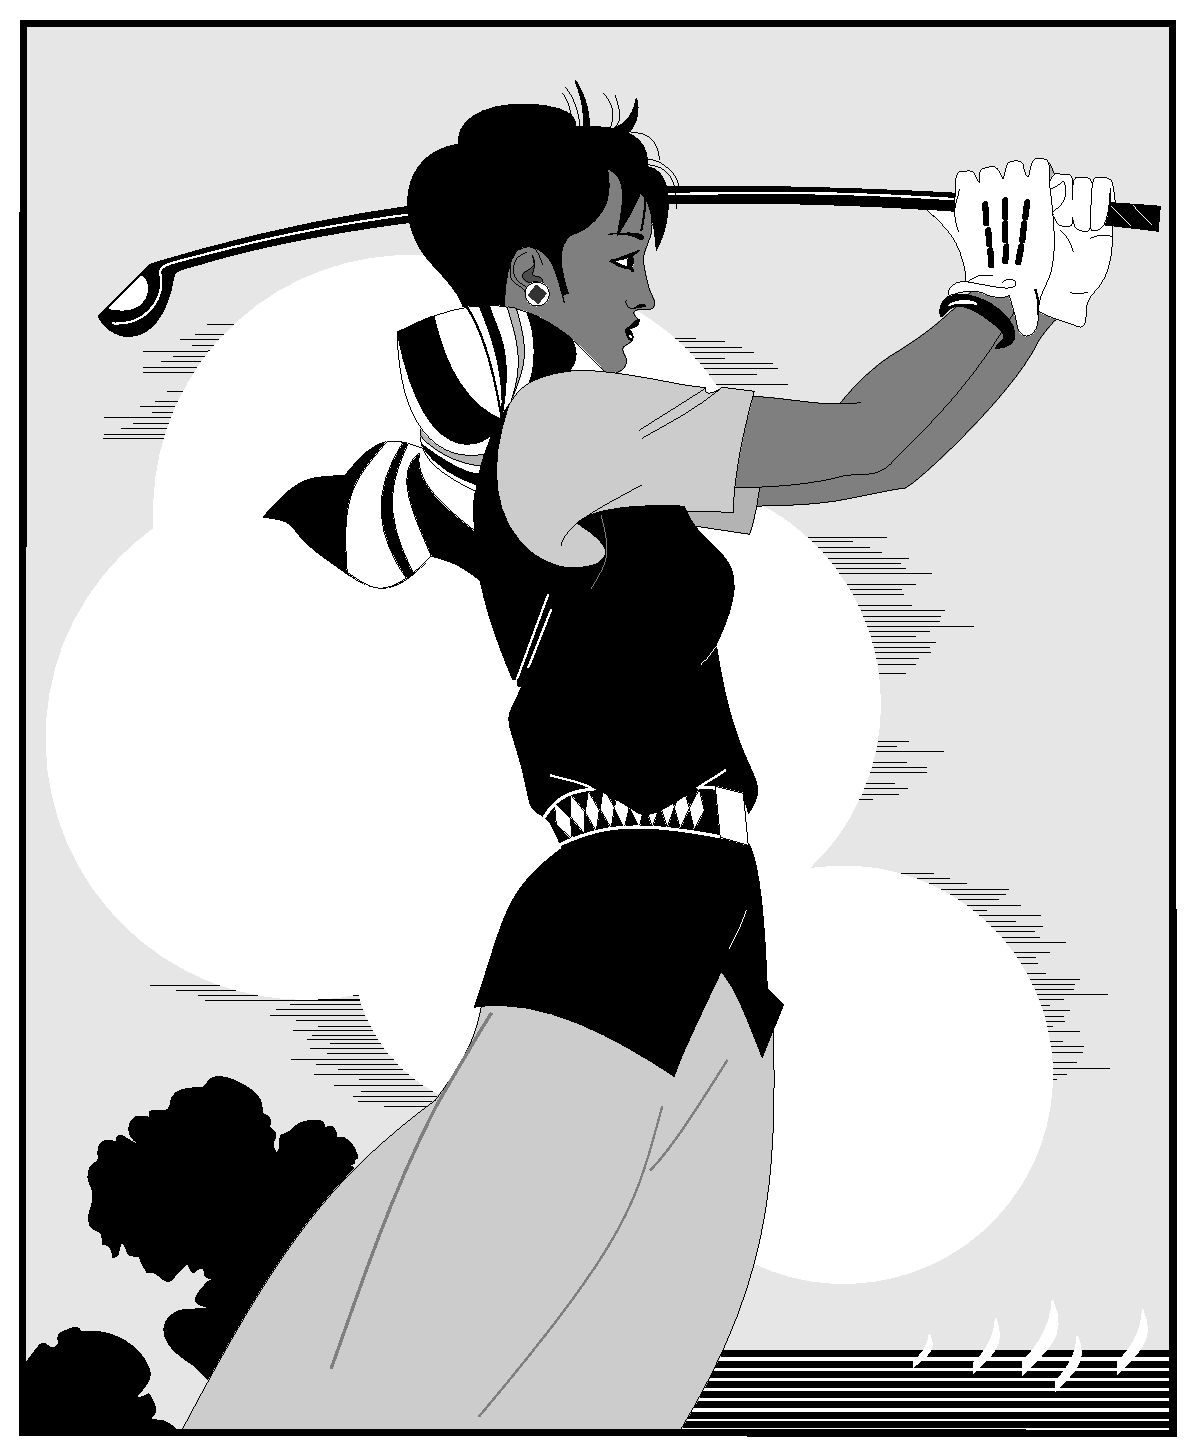
\includegraphics[width = 0.4\textwidth]{golfer}
%\bicaption[golfer5]{}{\xiaosi[0]打高尔夫球的人}{Fig.$\!$}{The person playing golf}\vspace{-1em}
\caption{\xiaosi[0]打高尔夫球的人}
\end{figure}

附录中公式的示例:
\begin{align}
a & = b \times c \\
E & = m c^2
\label{eq}
\end{align}

\chapter{这个星球上最好的免费Linux软件列表}[List of the Best Linux Software in our Planet]
\section{系统}

\href{http://fvwm.org/}{FVWM 自从上世纪诞生以来,此星球最强大的窗口管理器。}
推荐基于FVWM的桌面设计hifvwm:\href{https://github.com/dustincys/hifvwm}{https://github.com/dustincys/hifvwm}。

\subsection{hifvwm的优点}

\begin{enumerate}
	\item 即使打开上百个窗口也不会“蒙圈”。计算机性能越来越强大,窗口任务的管理必须要升级到打怪兽级别。
	\item 自动同步Bing搜索主页的壁纸。每次电脑开机,午夜零点自动更新,用户
		也可以手动更新,从此审美再也不疲劳。
	\item 切换窗口自动聚焦到最上面的窗口。使用键盘快捷键切换窗口时候,减少
		操作过程,自动聚焦到目标窗口。这一特性是虚拟窗口必须的人性化设
		计。
	\item 类似window右下角的功能的最小化窗口来显示桌面的功能此处类似
		win7/win10,实现在一个桌面之内操作多个任务。
	\item 任务栏结合标题栏。采用任务栏和标题栏结合,节省空间。
	\item 同类窗口切换。可以在同类窗口之内类似alt-tab的方式切换。
	\item ……
\end{enumerate}

\section{其他}

\href{https://github.com/goldendict/goldendict}{goldendict 星球最强大的桌面字典。}

\href{https://github.com/yarrick/iodine}{iodine,“HIT-WLAN + 锐捷”时代的福音。}

\href{http://www.aircrack-ng.org/}{aircrack,Wifi“安全性评估”工具。}

\href{https://www.ledger-cli.org/}{ledger,前“金融区块链”时代最好的复式记账系统。}

\href{https://orgmode.org/}{orgmode,最强大的笔记系统,从来没有之一。}

\href{https://www.jianguoyun.com/}{坚果云,国内一款支持WebDav的云盘系统,国内真正的云盘没有之一。}

\href{http://www.mutt.org/}{mutt, ``All mail clients suck. This one just sucks less.''}

\section{vim}
实现中英文每一句一行,以及实现每一句折叠断行的简单正则式,tex源码更加乖乖。
\begin{lstlisting}
vnoremap <leader>fae J:s/[.!?]\zs\s\+/\="\r".matchstr(getline('.'), '^\s*')/g<CR>
vnoremap <leader>fac J:s/[。!?]/\=submatch(0)."\n".matchstr(getline('.'), '^\s*')/g<CR>
vnoremap <leader>fle :!fmt -80 -s<CR>
\end{lstlisting}

\end{appendix}
%%% publications
%%% ---------------------------------------------------------------------------
%\pdfbookmark{Publications}{pdf:Publications}
\addchap{Publications}
Some ideas and figures have appeared previously in the following publications:

\bigskip

Put your publications here. You might consider using the \texttt{biblatex} package, for example with the following code:

\begin{verbatim}
\begin{refsection}
\nocite{publication_1,publication_2}
\setlength{\bibitemsep}{.5\baselineskip}
\setlength{\bibhang}{0pt}
\printbibliography[heading=none]
\end{refsection}
\end{verbatim}    % 所发文章
\begin{ceindex}
  %如果想要手动加索引,注释掉以下这一样,用wordlist环境
\printsubindex*
\end{ceindex}
    % 索引, 根据自己的情况添加或者不添加,选择自动添加或者手工添加。
\authorization %授权
%\authorization[saomiao.pdf] %添加扫描页的命令,与上互斥
% !TEX root = ../main.tex

% 致谢
\begin{acknowledgements}
衷心感谢导师~XXX~教授对本人的精心指导。他的言传身教将使我终生受益。

……

感谢哈深\LaTeX{}论文模板\hitszthesis\ !

\end{acknowledgements}
 %致谢
% !Mode:: "TeX:UTF-8" 

\begin{resume}
XXXX~年~XX~月~XX~日出生于~XXXX。

XXXX~年~XX~月考入~XX~大学~XX~院(系)XX~专业,XXXX~年~XX~月本科毕业并获得~XX~学学士学位。

XXXX~年~XX~月------XXXX~年~XX~月在~XX~大学~XX~院(系)XX~学科学习并获得~XX~学硕士学位。

XXXX~年~XX~月------XXXX~年~XX~月在~XX~大学~XX~院(系)XX~学科学习并获得~XX~学博士学位。

获奖情况:如获三好学生、优秀团干部、X~奖学金等(不含科研学术获奖)。

工作经历:

\textbf{( 除全日制硕士生以外,其余学生均应增列此项。个人简历一般应包含教育经历和工作经历。)}
\end{resume}
          % 博士学位论文有个人简介

%本科书序为:
% \chapter{The conclusion}

   % 结论
% \bibliographystyle{hithesis}
% \bibliography{reference}
% \authorization %授权
% % \authorization[saomiao.pdf] %添加扫描页的命令,与上互斥
% % !TEX root = ../main.tex

% 致谢
\begin{acknowledgements}
衷心感谢导师~XXX~教授对本人的精心指导。他的言传身教将使我终生受益。

……

感谢哈深\LaTeX{}论文模板\hitszthesis\ !

\end{acknowledgements}
 %致谢
% \begin{appendix}%附录
% % % !TEX root = ../main.tex

% 附录1
\chapter{外文资料的调研阅读报告或书面翻译}

\title{英文资料的中文标题}

{\heiti 摘要:} 本章为外文资料翻译内容。如果有摘要可以直接写上来,这部分好像没有
明确的规定。

\section{单目标规划}
北冥有鱼,其名为鲲。鲲之大,不知其几千里也。化而为鸟,其名为鹏。鹏之背,不知其几
千里也。怒而飞,其翼若垂天之云。是鸟也,海运则将徙于南冥。南冥者,天池也。
\begin{equation}\tag*{(123)}
 p(y|\mathbf{x}) = \frac{p(\mathbf{x},y)}{p(\mathbf{x})}=
\frac{p(\mathbf{x}|y)p(y)}{p(\mathbf{x})}
\end{equation}

吾生也有涯,而知也无涯。以有涯随无涯,殆已!已而为知者,殆而已矣!为善无近名,为
恶无近刑,缘督以为经,可以保身,可以全生,可以养亲,可以尽年。

\subsection{线性规划}
庖丁为文惠君解牛,手之所触,肩之所倚,足之所履,膝之所倚,砉然响然,奏刀騞然,莫
不中音,合于桑林之舞,乃中经首之会。
\begin{table}[ht]
\centering
  \centering
  \caption*{表~1\hskip1em 这是手动编号但不出现在索引中的一个表格例子}
  \label{tab:badtabular3}
  \begin{tabular}[c]{|m{1.5cm}|c|c|c|c|c|c|}\hline
    \multicolumn{2}{|c|}{Network Topology} & \# of nodes &
    \multicolumn{3}{c|}{\# of clients} & Server \\\hline
    GT-ITM & Waxman Transit-Stub & 600 &
    \multirow{2}{2em}{2\%}&
    \multirow{2}{2em}{10\%}&
    \multirow{2}{2em}{50\%}&
    \multirow{2}{1.2in}{Max. Connectivity}\\\cline{1-3}
    \multicolumn{2}{|c|}{Inet-2.1} & 6000 & & & &\\\hline
    & \multicolumn{2}{c|}{ABCDEF} &\multicolumn{4}{c|}{} \\\hline
\end{tabular}
\end{table}

文惠君曰:“嘻,善哉!技盖至此乎?”庖丁释刀对曰:“臣之所好者道也,进乎技矣。始臣之
解牛之时,所见无非全牛者;三年之后,未尝见全牛也;方今之时,臣以神遇而不以目视,
官知止而神欲行。依乎天理,批大郤,导大窾,因其固然。技经肯綮之未尝,而况大坬乎!
良庖岁更刀,割也;族庖月更刀,折也;今臣之刀十九年矣,所解数千牛矣,而刀刃若新发
于硎。彼节者有间而刀刃者无厚,以无厚入有间,恢恢乎其于游刃必有余地矣。是以十九年
而刀刃若新发于硎。虽然,每至于族,吾见其难为,怵然为戒,视为止,行为迟,动刀甚微,
謋然已解,如土委地。提刀而立,为之而四顾,为之踌躇满志,善刀而藏之。”

文惠君曰:“善哉!吾闻庖丁之言,得养生焉。”


\subsection{非线性规划}
孔子与柳下季为友,柳下季之弟名曰盗跖。盗跖从卒九千人,横行天下,侵暴诸侯。穴室枢
户,驱人牛马,取人妇女。贪得忘亲,不顾父母兄弟,不祭先祖。所过之邑,大国守城,小
国入保,万民苦之。孔子谓柳下季曰:“夫为人父者,必能诏其子;为人兄者,必能教其弟。
若父不能诏其子,兄不能教其弟,则无贵父子兄弟之亲矣。今先生,世之才士也,弟为盗
跖,为天下害,而弗能教也,丘窃为先生羞之。丘请为先生往说之。”

柳下季曰:“先生言为人父者必能诏其子,为人兄者必能教其弟,若子不听父之诏,弟不受
兄之教,虽今先生之辩,将奈之何哉?且跖之为人也,心如涌泉,意如飘风,强足以距敌,
辩足以饰非。顺其心则喜,逆其心则怒,易辱人以言。先生必无往。”

孔子不听,颜回为驭,子贡为右,往见盗跖。

\subsection{整数规划}
盗跖乃方休卒徒大山之阳,脍人肝而餔之。孔子下车而前,见谒者曰:“鲁人孔丘,闻将军
高义,敬再拜谒者。”谒者入通。盗跖闻之大怒,目如明星,发上指冠,曰:“此夫鲁国之
巧伪人孔丘非邪?为我告之:尔作言造语,妄称文、武,冠枝木之冠,带死牛之胁,多辞缪
说,不耕而食,不织而衣,摇唇鼓舌,擅生是非,以迷天下之主,使天下学士不反其本,妄
作孝弟,而侥幸于封侯富贵者也。子之罪大极重,疾走归!不然,我将以子肝益昼餔之膳。”%本科生翻译论文
% \end{appendix}

\end{document}

% Local Variables:
% TeX-engine: xetex
% End:
